\chapter{Fundamenta��o Te�rica}
\label{CHP:FUND}

Neste cap�tulo s�o descritos alguns fundamentos sobre modelos de falhas em mem�ria e os tipos de algoritmos mais discutidos na literatura. Tamb�m s�o apresentadas algumas caracter�sticas do gerenciador de mem�ria do Linux que s�o importantes para o projeto do diagn�stico.

    %%% Se��o 2.1 Modelagem de Falhas em Mem�rias:
    \section{Modelos de Falhas em Mem�rias}

%\subsection{Modelagem de Falhas}

Em sistemas computacionais, as palavras falha, erro e defeito possuem significados distintos. Suas diferen�as ser�o enunciadas como apresentadas por \cite{WEBER:2001}, para uma melhor contextualiza��o.

A falha (\emph{fault}) � um comportamento que ocorre no n�vel mais baixo do sistema. Geralmente est� associada ao \emph{hardware} ou � escrita do c�digo. Por exemplo, uma flutua��o na fonte de alimenta��o ou a troca de um ``>='' por um ``>'' pode causar uma falha. Assim, estas est�o associadas ao universo f�sico, conforme ilustrado na Figura \ref{FIG:FED}.

O erro (\emph{error}) � a representa��o da falha no universo da informa��o. Ele se apresenta quando, por conseq��ncia de uma falha, a informa��o for corrompida. Quando um estado pode levar a ocorr�ncia de um defeito, pode-se dizer que o sistema est� em estado de erro.

O defeito (\emph{failure}) � um desvio da especifica��o, e ocorre em conseq��ncia de um erro. O defeito � algo percebido pelo usu�rio, por isso os defeitos est�o associados ao universo do usu�rio.

%Uma falha n�o necessariamente leva a um estado de erro, pois a linha de c�digo com falha pode nunca ser executada. Um erro tamb�m n�o necessariamente leva a um estado de defeito, pois talvez uma informa��o nunca seja usada.

\begin{figure}[!ht]
\centering
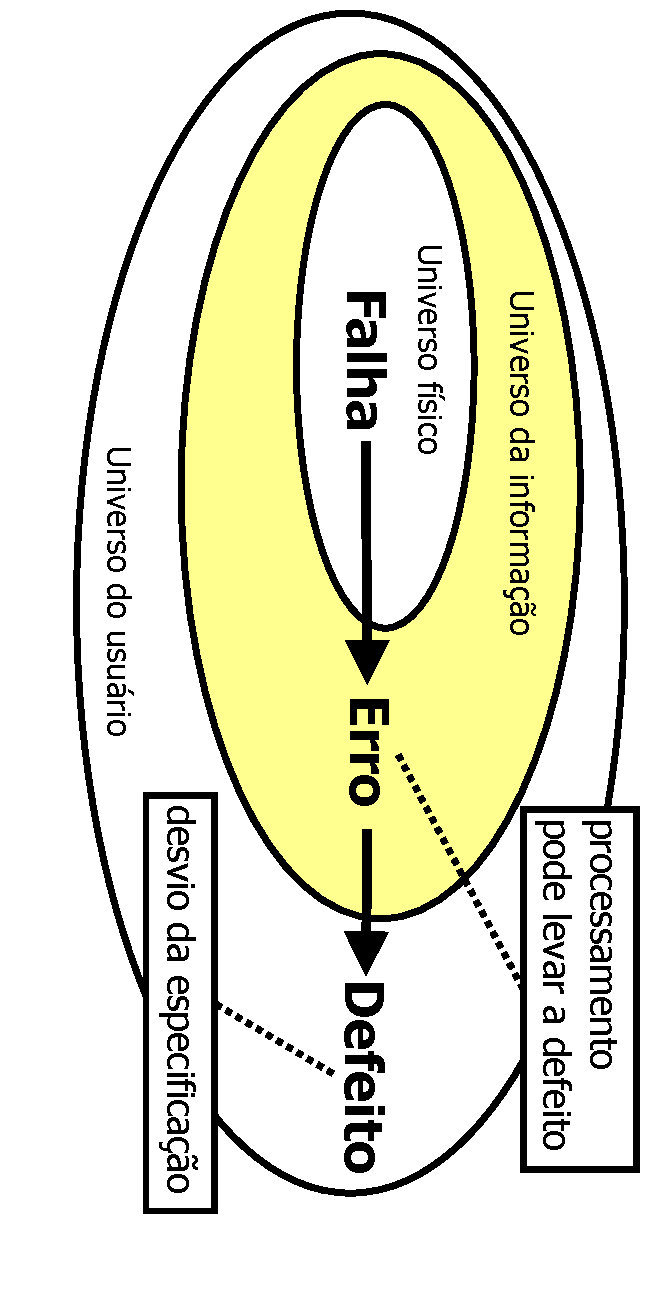
\includegraphics[height = 0.7 \linewidth, angle = 90]{figs/falha_erro_defeito.pdf}
\caption[Falha, erro e defeito]{Modelo de tr�s universos \cite{WEBER:2001}.}
\label{FIG:FED}
\end{figure}

Por exemplo, um chip de mem�ria que apresenta uma falha em um de seus bits (falha, universo f�sico) pode provocar uma interpreta��o errada da informa��o armazenada em uma estrutura de dados (erro, universo da informa��o) e como resultado o sistema pode negar autoriza��o de embarque para todos os passageiros de um v�o (defeito, universo do usu�rio).
� interessante observar que uma falha n�o leva, necessariamente, a um erro (aquela por��o da mem�ria pode nunca ser usada) e um erro n�o leva, necessariamente, a um defeito (no exemplo, a informa��o de v�o lotado poderia eventualmente ser obtida a partir de outros dados redundantes da estrutura).

Neste trabalho ser� utilizado apenas o conceito de falha, pois estamos interessados em diagnosticar um \emph{hardware}, parte do universo f�sico.

A descri��o de como alguma coisa pode falhar � o modelo de falha \cite{ADAMS:2003}. Esta descri��o pode ser feita em v�rios n�veis de abstra��o. No caso de circuitos integrados, existem os n�veis comportamental, funcional, l�gico, el�trico e geom�trico, mostrados na Figura \ref{FIG:ABSTRACTION}.

\begin{figure}[!ht]
\centering
\includegraphics[width = 0.7 \linewidth]{figs/abstraction_levels.png}
\caption[N�veis de abstra��o de falhas]{N�veis de abstra��o para modelagem de falhas.} \label{FIG:ABSTRACTION}
\end{figure}

O n�vel mais alto de abstra��o � o comportamental, que visa fazer uma descri��o em alto n�vel do sistema, geralmente auxiliada por uma \ac{HDL}.

Na modelagem em n�vel funcional, os circuitos s�o vistos como caixas pretas, isto �, apenas as entradas e sa�das s�o consideradas, n�o importando o trabalho interno realizado. Historicamente, esta � a modelagem mais utilizada para testes de mem�ria \cite{ADAMS:2003}.

No n�vel l�gico mais detalhes s�o acrescentados, passando a serem consideradas as portas l�gicas que comp�em os circuitos. Abaixo, est� o n�vel el�trico, onde as falhas s�o vistas nas opera��es dos transistores. Por fim, o modelo geom�trico se refere a todos os detalhes do processo de fabrica��o do circuito integrado, como tamanho e localiza��o das portas, dist�ncia entre c�lulas adjacentes, correntes de fuga entre po�os de dopagem, dentre outros \cite{ADAMS:2003}.

Os modelos de falhas funcionais s�o os mais empregados em testes e diagn�sticos de mem�ria \cite{ADAMS:2003}, porque n�o h� interesse na natureza das falhas, mas no seu efeito na funcionalidade dos circuitos. A partir deste ponto trataremos as falhas sempre a n�vel funcional.

%\subsection{Modelagem de Falhas em Mem�rias}

Os modelos de falhas cl�ssicos para circuitos digitais s�o \emph{Stuck-At Fault}, \emph{Bridging Fault}, \emph{Open Fault} e \emph{Delay Fault}. No entanto, eles n�o s�o suficientes para representar todas as falhas importantes em mem�rias, fazendo-se necess�rio definir erros mais espec�ficos para este tipo de circuito \cite{NAIR:1978, PAPACHRISTOU:1985}.

As falhas em mem�rias podem ser classificadas em tr�s categorias: falhas nas c�lulas de mem�ria, falhas no decodificador de endere�o e falhas din�micas. Cada umas destas categorias ser�o descritas nas pr�ximas se��es.

\subsection{Falhas na Matriz de C�lulas de Mem�ria}

As falhas nas c�lulas acontecem principalmente devido a curtos de metaliza��o e acoplamento capacitivo \cite{THATTE:1977}. Os principais tipos s�o \ac{SAF}, \ac{TF}, \ac{CF} e \ac{NPSF}, que s�o detalhados adiante.

Para descrever os estados das c�lulas de mem�ria com ou sem falhas, uma boa maneira � utilizar diagramas de Markov \cite{DAVID:1989}. Esses diagramas descrevem o comportamento de sistemas em um espa�o estado-tempo. Uma c�lula livre de qualquer defeito pode receber uma opera��o de escrita para qualquer estado e, quando lida, ret�m a informa��o na c�lula. A Figura \ref{FIG:MARKOV:FAUL_FREE} mostra o diagrama de Markov para uma c�lula de mem�ria livre de falhas. Adota-se neste trabalho a nota��o utilizada em \cite{ADAMS:2003}, onde as transi��es de estado representam as opera��es e $S_0$ e $S_1$ indicam que a c�lula est� no estado 0 ou 1, respectivamente. A transi��o R indica uma opera��o de leitura e W0 e W1 indicam opera��es de escrita para o estado 0 e 1, respectivamente.

\begin{figure}[!ht]
\centering
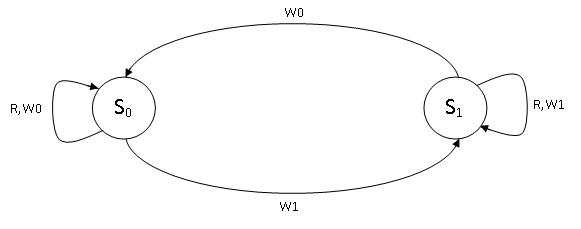
\includegraphics[width = 0.7 \linewidth]{figs/markov_fault_free.png}
\caption[Diagrama de c�lula sem falhas]{Diagrama de Markov para uma c�lula de mem�ria sem falhas. \cite{ADAMS:2003}} \label{FIG:MARKOV:FAUL_FREE}
\end{figure}

\subsubsection{\emph{Stuck-At Fault}}

Entre os modelos cl�ssicos de falhas em mem�rias, o mais conhecido e tamb�m o mais simples � o modelo \ac{SAF}, que � utilizado para indicar que uma c�lula est� presa em um determinado estado. A Figura ~\ref{FIG:MARKOV:SAFS} mostra o diagrama de Markov de uma falha do tipo \ac{SAF}. Independente do evento que ocorra, a c�lula se mant�m no seu estado atual.

\begin{figure}[!ht]
\centering
\subfigure[\label{FIG:MARKOV:STUCKAT_0}]{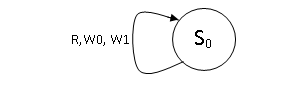
\includegraphics[width = 0.4 \linewidth]{figs/markov_stuckat_0.png}}
\subfigure[\label{FIG:MARKOV:STUCKAT_1}]{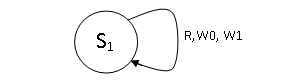
\includegraphics[width = 0.4 \linewidth]{figs/markov_stuckat_1.png}}
\caption[Diagramas \emph{Stuck-At}]{Diagramas de uma c�lula de mem�ria com \emph{Sutck-At} 0 (a) e \emph{Stuck-At} 1 (b). \cite{ADAMS:2003}} \label{FIG:MARKOV:SAFS}
\end{figure}

\subsubsection{Transition Fault}

Outro modelo simples de falha � o modelo \ac{TF}. De certa forma ele se parece com o \ac{SAF}, mas no caso de uma c�lula de mem�ria, ela ir� reter ambos os estados, mas uma vez escrita para um estado, ela n�o poder� fazer a transi��o de volta. Assim, quando a mem�ria � energizada a c�lula pode estar no estado ``0'' ou ``1'' e s� pode ser escrita em uma dire��o. A Figura ~\ref{FIG:MARKOV:TR} mostra o diagrama de Markov para uma falha do tipo \ac{TF}.

\begin{figure}[!ht]
\centering
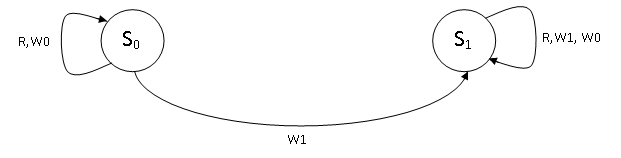
\includegraphics[width = 0.7 \linewidth]{figs/markov_transition.png}
\caption[Diagrama de \emph{Transition Fault}]{Diagrama de uma c�lula com \emph{Transition Fault}. \cite{ADAMS:2003}} \label{FIG:MARKOV:TR}
\end{figure}

\subsubsection{Coupling Fault}
\label{SEC:R3CF}

Para ilustrar uma \ac{CF} � necess�rio introduzir o diagrama de Markov para duas c�lulas. A Figura \ref{FIG:MARKOV:2FREE} mostra um par de c�lulas livres de falha, representadas pelos �ndices $i$ e $j$. Cada c�lula pode ser individualmente lida ou escrita para cada estado independentemente da outra, havendo um total de quatro estados poss�veis para o conjunto.

\begin{figure}[!ht]
\centering
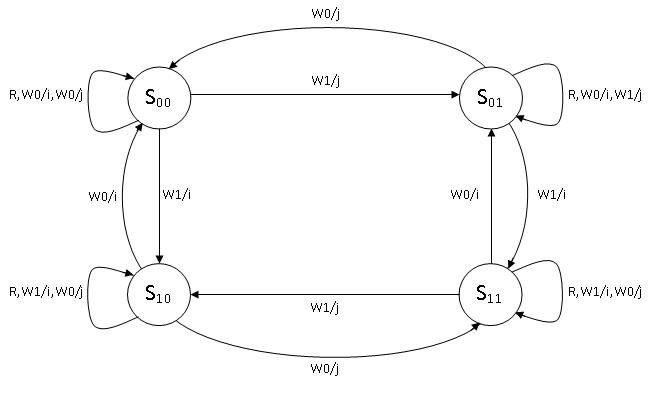
\includegraphics[width = 0.8 \linewidth]{figs/markov_2_cell.png}
\caption[Diagrama para duas c�lulas]{Diagrama para duas c�lulas sem falhas. \cite{ADAMS:2003}} \label{FIG:MARKOV:2FREE}
\end{figure}

Utiliza-se o modelo de falhas \ac{CF}, ou simplesmente acoplamento, quando h� um ou mais pares de c�lulas eletricamente acoplados, isto �, quando h� interfer�ncia eletromagn�tica entre elas. De forma simplificada, uma c�lula pode estar acoplada as c�lulas da sua vizinhan�a causando a transi��o para um estado err�neo ou uma falsa transi��o.

Os principais fatores que causam a falha \ac{CF} s�o a capacit�ncia m�tua e a corrente de fuga de uma c�lula para outra \cite{SUK:1981}. Papachristou \cite{PAPACHRISTOU:1985} a definiu formalmente como:
\begin{quote}
Quando uma opera��o de escrita que afeta a transi��o de 0 para 1 ou de 1 para 0 na c�lula $j$ muda o estado de outra c�lula $i$ ($i \neq j$), independente do conte�do da outra c�lula. Isto n�o implica que uma transi��o em $i$ mude o estado de $j$.
\end{quote}

Quando h� uma falha \ac{CF} entre as c�lulas, o diagrama de Markov do par passa a ser representado pela Figura \ref{FIG:MARKOV:CF}. Como descrito na defini��o, � poss�vel haver \ac{CF} em apenas um sentido, onde a c�lula provoca a falha na outra mas o oposto n�o acontece. No caso ilustrado, a falha s� ocorre quando a c�lula $i$ est� no estado 0 e a c�lula $j$ faz uma transi��o de 0 para 1. Caso a c�lula $i$, ao inv�s da $j$, fa�a uma transi��o de 0 para 1, nenhuma falha ser� provocada. A c�lula que causa a \ac{CF} � chamada de c�lula agressora \cite{ADAMS:2003} ou acopladora \cite{PAPACHRISTOU:1985} e a c�lula que sofre a falha � chamada de v�tima ou acoplada.
%??? precisa referenciar nos 2 momentos? ou s� no 2o? ou como est� mesmo?

\begin{figure}[!ht]
\centering
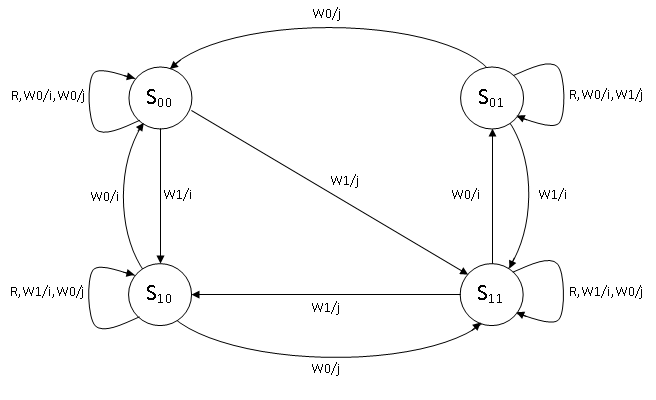
\includegraphics[width = 0.8 \linewidth]{figs/markov_coupling.png}
\caption[Diagrama de \emph{Coupling fault}]{Diagrama para duas c�lulas com \ac{CF}. \cite{ADAMS:2003}} \label{FIG:MARKOV:CF}
\end{figure}

A falha \ac{CF} pode se apresentar nos seguinte tipos \cite{RAGHURAMAN:2005}:

\begin{enumerate}
  \item \textbf{Inversion Coupling Fault}: Uma transi��o na c�lula agressora inverte o conte�do da c�lula v�tima;
  \item \textbf{Idempotent Coupling Fault}: Uma transi��o na c�lula agressora for�a um valor l�gico fixo na c�lula v�tima;
  \item \textbf{State Coupling Fault}: A c�lula v�tima � for�ada para certo estado apenas se a c�lula agressora estiver em  determinado estado. Tamb�m conhecida como \ac{PSF}.
\end{enumerate}

Um conjunto de $k$ c�lulas � dito estar $k$-acoplado (\emph{$k$-coupled}) se uma transi��o em uma c�lula causa uma transi��o em outra c�lula do conjunto quando as outras $k-2$ c�lulas est�o em certo estado. Um caso especial chamado de \emph{restricted $k$-coupling} � convenientemente definido como um \emph{$k$-coupling} onde as $k-1$ c�lulas n�o possuem acoplamento entre si. Devido a enorme complexidade dos modelos de falhas para $k$ maior que 3, apenas falhas \emph{2-coupling} e \emph{restricted 3-coupling} t�m sido investigadas na literatura \cite{PAPACHRISTOU:1985} \cite{ADAMS:2003}.

\subsubsection{Neighborhood Pattern Sensitive Fault}

O modelo \ac{NPSF}, se apresenta sobre uma c�lula chamada de c�lula-base e sua vizinhan�a f�sica. Na realidade, o \ac{NPSF} � um caso especial de \emph{$k$-coupling} em que as $k-1$ c�lulas agressoras est�o restritas a uma vizinhan�a fixa em proximidade f�sica da c�lula base. Este modelo � bastante estudado por ser mais comum que acoplamentos entre c�lulas distantes \cite{PETRU:2002}.

\subsection{Falhas no Decodificador de Endere�o}

O decodificador � um circuito de l�gica combinacional simples que seleciona uma �nica c�lula de mem�ria para um dado endere�o. Qualquer falha ocorrida no decodificador far� com que ele se comporte de umas das maneiras:

\begin{enumerate}
  \item O decodificador n�o ir� acessar a c�lula endere�ada. Al�m disto, ele pode acessar c�lulas n�o endere�adas;
  \item O decodificador ir� acessar m�ltiplas c�lulas, incluindo a c�lula endere�ada.
\end{enumerate}

No caso de m�ltiplos acessos (ii), podemos ver a falha como uma falha na matriz de c�lulas, isto �, como uma \ac{CF} entre as c�lulas afetadas. No caso (i), a c�lula que deveria ter sido selecionada pode ser vista como \emph{stuck at} 0 ou \emph{stuck at} 1, dependendo da l�gica utilizada.

Em todos os casos, podemos visualizar as falhas no decodificador como falhas na matriz de c�lulas da mem�ria \cite{NAIR:1978} \cite{PETRU:2002}.

\subsection{Falhas Din�micas}

As falhas din�micas em mem�rias s�o tamb�m chamadas de falhas na l�gica de escrita e leitura (\emph{Read/Write Logic Fault}). Algumas linhas dos circuitos de escrita e leitura podem estar em \emph{stuck at} 0 ou \emph{stuck at} 1. Neste caso, podemos considerar a falha como uma \ac{SAF} nas c�lulas afetadas por essas linhas. As linhas de entrada ou sa�da de dados das c�lulas podem conter curtos ou acoplamentos capacitivos entre elas. Estas falhas podem ser visualizadas como \ac{CF} entre as c�lulas correspondentes.

Portanto, para testes de \ac{RAM}, todas os tipos de falhas podem ser representados apenas pelos modelos de falhas na matriz de c�lulas de mem�ria, isto � \ac{SAF}, \ac{TF}, \ac{CF} e \ac{NPSF} \cite{NAIR:1978,PETRU:2002}. 
    %%% Se��o 2.2 Tipos de testes de mem�ria:
    \section{Tipos de testes de mem�ria}
\label{SEC:TESTES}

Uma mem�ria guarda zeros e uns. Se zeros s�o escritos em todos os endere�os da mem�ria e lidos de todos os endere�os, ent�o metade das falhas foram cobertas, certo? Na realidade, n�o.

O teste mencionado � um dos testes mais simples existentes. � chamado de padr�o zero-um (\emph{zero-one pattern}) ou padr�o trivial. %Apesar da simplicidade, este teste tem cobertura de 100\% das falhas \ac{SAF}, por�m � incapaz de detectar a maior parte dos outros modelos \cite{ADAMS:2003}.
Apesar da simplicidade e deste teste ter cobertura de 100\% das falhas \ac{SAF}, ele � incapaz de detectar a maior parte dos outros tipos de falhas \cite{ADAMS:2003}. A situa��o descrita na Figura \ref{FIG:ARRAY_NO_01} � um exemplo onde este teste n�o � suficiente. Neste caso h� uma falha nos decodificadores de forma que, independente do endere�o selecionado, sempre a mesma c�lula � acessada, tanto na escrita quanto na leitura.

\begin{figure}[!htb]
\centering
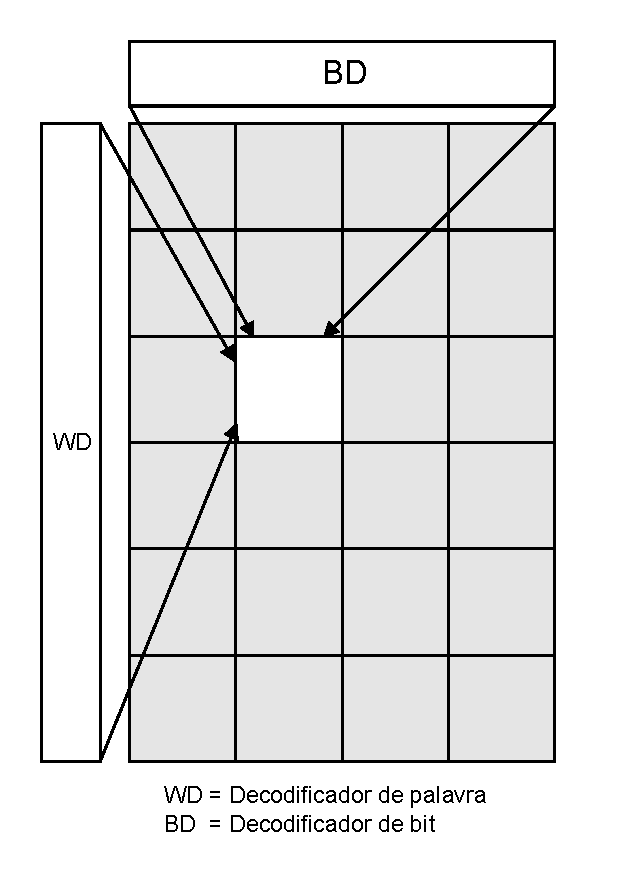
\includegraphics[width = 0.6 \linewidth]{figs/array_no_01.pdf}
\caption[Erro n�o detect�vel por padr�o zero-um]{Erro n�o detect�vel por padr�o zero-um.} \label{FIG:ARRAY_NO_01}
\end{figure}

Para que seja poss�vel testar mem�rias de forma mais completa, � necess�rio usar uma combina��o de padr�es de teste (\emph{patterns}), onde cada padr�o tem a capacidade de detectar certos tipos de falhas. Nenhum padr�o sozinho � suficiente para testar uma mem�ria por completo \cite{DEAN:1994}. Padr�es s�o a ess�ncia dos testes de mem�ria \cite{ADAMS:2003}.

Para a descri��o de testes, adota-se uma nota��o baseada em \cite{ADAMS:2003}. A Tabela \ref{TAB:01} mostra a representa��o do teste zero-um citado anteriormente. Cada linha indica uma sequ�ncia de opera��es que deve ser aplicada a cada c�lula antes de prosseguir para a pr�xima sequ�ncia. A estas sequ�ncias, tamb�m d�-se o nome de elementos de teste \cite{PAPACHRISTOU:1985}. No exemplo temos quatro elementos, do 1 ao 4, cada um com apenas uma opera��o. As opera��es podem ser:

\begin{itemize}
  \item W0 escrever 0 na c�lula
  \item R0 ler estado da c�lula, esperado 0
  \item W1 escrever 1 na c�lula
  \item R1 ler estado da c�lula, esperado 1
\end{itemize}

Ao final das opera��es em um endere�o, a passagem de uma c�lula para outra pode ser de forma ascendente, representada pelo s�mbolo $\Uparrow$, descendente, representada por $\Downarrow$ ou em qualquer dire��o, representada por $\Updownarrow$.

\begin{table}[!ht]
\caption{\emph{Zero-Ones Pattern.}}
\centering
\label{TAB:01}
\begin{tabular}{| c | l r |}
\hline
1 & W0 & $\Updownarrow$ \\
2 & R0 & $\Updownarrow$ \\
3 & W1 & $\Updownarrow$ \\
4 & R1 & $\Updownarrow$ \\
\hline
\end{tabular}
\end{table}

%A Complexidade de um algoritmo consiste na quantidade de trabalho necess�ria para a sua execu��o, expressa em fun��o das opera��es fundamentais, as quais variam de acordo com o algoritmo, e em fun��o do volume de dados. � medida segundo um modelo matem�tico que sup�e que este vai trabalhar sobre uma entrada (massa de dados) de tamanho N. O processo de execu��o de um algoritmo pode ser dividido em etapas elementares denominadas passos (n�mero fixo de opera��es b�sicas, tempo constante, opera��o de maior freq��ncia chamada dominante). O n�mero de passos de um algoritmo � considerado como o n�mero de execu��es da opera��o dominante em fun��o das sa�das, desprezando-se constantes aditivas ou multiplicativas.

Atrav�s desta drescri��o tamb�m � possivel medir a complexidade do teste. Isto �, quantos ciclos s�o necess�rios para executar todo o teste. Supondo que uma opera��o de escrita ou leitura possa ser realizada em um ciclo, o teste apresentado possui uma complexidade 4$N$, onde $N$ � a quantidade de c�lulas ou o tamanho da mem�ria. Este teste � dito ser de ordem $N$, representado por $O(N)$. Um teste de complexidade 14$N\log_2(N)$ possui ordem $O(N\log_2(N))$. O conceito de complexidade � importante pois os chips de mem�ria crescem constantemente seguindo a Lei de Moore. Isto faz com que testes mais complexos levem tempos impratic�veis para os tamanhos e velocidades das mem�rias atuais.

Tomando como exemplo uma mem�ria com tempo de acesso de 1,25 ns\footnote{Tempo de acesso retirado do \emph{datasheet} de uma mem�ria DDR3 SDRAM SODIMM. \cite{MICRON:2008}.}, a Tabela \ref{TAB:TEMPOS} mostra os tempos de execu��o de supostos testes de diferentes complexidades em diferentes tamanhos de mem�ria.

\begin{table}[!ht]
\caption{Tempos de execu��o em mem�ria com tempo de acesso de 1,25 ns.}
\centering
\label{TAB:TEMPOS}
\begin{tabular}{|l|l|l|l|l|}
\hline
Tamanho & \multicolumn{4}{c|}{Complexidade} \\
\cline{2-5}
$N$ & $N$ & $N\log_2(N)$ & $N^{3/2}$ & $N^2$ \\
\hline
1 KB & 1,28 $\mu$s & 12,8 $\mu$s & 40,96 $\mu$s & 1,31 ms \\
4 KB & 5,12 $\mu$s &  61,44 $\mu$s & 327,68 $\mu$s & 20,97 ms \\
16 KB & 20,48 $\mu$s & 286,72 $\mu$s & 2,62 ms & 335,54 ms \\
64 KB & 81,92 $\mu$s & 1,31 ms & 20,97 ms & 5,37 s \\
256 KB & 327,68 $\mu$s & 5,90 ms & 167,77 ms &  1,43 min \\
1 MB & 1,31 ms & 26,21 ms & 1,34 s &  22,91 min \\
4 MB & 5,24 ms & 115,34 ms & 10,74 s &  6,11 h \\
16 MB & 20,97 ms & 503,32 ms &  1,43 min &  4,07 dias \\
64 MB & 83,89 ms & 2,18 s &  11,45 min &  65,16 dias \\
256 MB & 335,54 ms & 9,40 s &  1,53 h &  2,86 anos \\
1 GB & 1,34 s & 40,27 s &  12,22 h &  45,70 anos \\
2 GB & 2,68 s & 1,39 min &  1,44 dia &  182,79 anos \\
4 GB & 5,37 s & 2,86 min &  4,07 dias &  731,18 anos \\
\hline
\end{tabular}
\end{table}

� importante notar que em testes reais os tempos s�o m�ltiplos desses valores. Um teste de complixadade 8$N$, por exemplo, iria levar $8 \cdot 1,34 s = 10,72 s$ para testar 1 GB de mem�ria, pois, pela tabela, leva-se $1,34 s$ para executar cada $N$ opera��es. Assim, apenas testes de complexidade at� $O(N\log_2(N))$ s�o aceit�veis \cite{RAGHURAMAN:2005}.

Os padr�es de testes de mem�ria s�o comumente categorizados como caminhantes (\emph{walking}), marchantes (\emph{marching}) e galopantes (\emph{galloping}) \cite{VANDEGOOR:1998}.

\subsubsection{Testes Caminhantes (\emph{Walking})}

Um teste � dito ser caminhante (\emph{walking}) quando, em cada momento, h� apenas uma c�lula em um estado diferente de todas as outras.

Inicialmente a mem�ria � totalmente preenchida com um padr�o, ent�o as opera��es de escrita e leitura s�o realizadas em uma c�lula e ao final da sequ�ncia, a c�lula deve voltar ao estado inicial. A tabela \ref{TAB:WALKING} mostra um exemplo de elemento para um teste caminhante.

\begin{table}[!ht]
\caption{Exemplo de \emph{walking}.}
\centering
\label{TAB:WALKING}
\begin{tabular}{| c | l r |}
\hline
1 & R0, W1, R1, W0 & $\Uparrow$ \\
\hline
\end{tabular}
\end{table}

O que caracteriza este elemento como caminhante � que a �ltima opera��o de escrita (W0) retorna a c�lula para o estado em que ela se encontrava antes do in�cio da sequ�ncia (que pode ser notado pela leitura R0).

\subsubsection{Testes Marchantes (\emph{Marching})}

Um padr�o em marcha (\emph{marching pattern}) � quando o teste muda o estado da c�lula testada e n�o a retorna para o estado anterior. Assim, antes de come�ar o teste, a mem�ria est� preenchida com um certo padr�o, ap�s uma sequ�ncia percorrer metade da mem�ria, metade estar� com o padr�o inicial e a outra metade estar� com o padr�o escrito pelo teste. Um exemplo de um elemento \emph{march} � mostrado na tabela \ref{TAB:MARCHING}.

\begin{table}[!ht]
\caption{Exemplo de \emph{marching}.}
\centering
\label{TAB:MARCHING}
\begin{tabular}{| c | l r |}
\hline
1 & R0, W1, R1 & $\Downarrow$ \\
\hline
\end{tabular}
\end{table}

O que diferencia este elemento de um caminhante � que sua �ltima escrita n�o � necessariamente para o valor inicial da c�lula.

\subsubsection{Testes Galopantes (\emph{Galloping})}

Enquanto os padr�es caminhantes e marchantes s�o orientados a dado, o galopante (\emph{galloping pattern}) � orientado a endere�o. A diferen�a � que esta categoria faz uma checagem do tipo \emph{ping-pong} entre a c�lula base (c�lula atualmente testada) e todas as outras da matriz. Como em cada opera��o � preciso percorrer toda a mem�ria, este tipo de teste leva muito tempo para ser realizado. Sua complexidade � da ordem de $O(N^2)$, o que � bastante, comparada a complexidade de ordem $N$ dos outros dois tipos apresentados.

A cobertura de falhas dos testes galopantes � consideravelmente maior, no entanto o excesso de tempo faz com que sua utiliza��o seja invi�vel. Como mostrado na Tabela \ref{TAB:TEMPOS}, um teste que levaria alguns minutos com padr�es caminhantes ou marchantes, poderia precisar de anos para ser conclu�do com um padr�o galopante.

\subsection{Testes Conhecidos}

Desde metade do s�culo XX muitos padr�es para testes de mem�ria t�m sido propostos. Ao longo do tempo eles foram aperfei�oados tanto no sentido de aprimorar a cobertura de falhas quanto no sentido de reduzir a quantidade de opera��es realizadas. Neste cap�tulo trataremos apenas dos algoritmos mais utilizados pela ind�stria e referenciados na literatura.

\subsubsection{S�rie March}

Existe um conjunto tradicional de testes do tipo marchante identificados por letras. Destes, o March C- ganhou destaque em muitos trabalhos por ser muito simples e ainda assim poderoso na detec��o de falhas. Seu nome � dado por ser uma otimiza��o de outro padr�o, chamado March C, onde algumas inefici�ncias foram eliminadas. Como pode ser visto na Tabela \ref{TAB:MARCHC-}, o March C- � um teste $10N$. Ele � capaz de detectar todas as falhas do tipo \ac{SAF}, \emph{idempotent} \ac{CF}, \ac{TF} e parte das falhas de alguns outro tipos \cite{ADAMS:2003}. De acordo com \cite{PETRU:2002}, 81,25\% das falhas \ac{CF} simples entre 2 c�lulas s�o detectadas por este teste.

\begin{table}[!ht]
\caption{\emph{March C- pattern.}}
\centering
\label{TAB:MARCHC-}
\begin{tabular}{| c | l r |}
\hline
1 & W0 & $\Updownarrow$ \\
2 & R0, W1 & $\Uparrow$ \\
3 & R1, W0 & $\Uparrow$ \\
4 & R0, W1 & $\Downarrow$ \\
5 & R1, W0 & $\Downarrow$ \\
6 & R0 & $\Updownarrow$ \\
\hline
\end{tabular}
\end{table}

Uma melhoria do March C- foi proposta por \cite{ADAMS:2003}. Chamado de Enhanced March C-, o teste, descrito na tabela \ref{TAB:EMARCHC-}, executa $18N$ opera��es e detecta algumas falhas al�m das j� cobertas pelo March C-.

\begin{table}[!ht]
\caption{\emph{Enhanced March C- pattern.}}
\centering
\label{TAB:EMARCHC-}
\begin{tabular}{| c | l r |}
\hline
1 & W0 & $\Updownarrow$ \\
2 & R0, W1, R1, W1 & $\Uparrow$ \\
3 & R1, W0, R0, W0 & $\Uparrow$ \\
4 & R0, W1, R1, W1 & $\Downarrow$ \\
5 & R1, W0, R0, W0 & $\Downarrow$ \\
6 & R0 & $\Updownarrow$ \\
\hline
\end{tabular}
\end{table}

\subsubsection{Moving Invertion}

Outro padr�o muito conhecido � o \ac{MOVI}. Seu funcionamento � um pouco mais complexo que os testes do tipo marchante.

Inialmente toda a mem�ria � preenchida com zeros. Ent�o repete-se o seguinte procedimeno: uma palavra � lida; um bit � escrito para 1; a palavra � lida novamente. Isto se repete at� que todos os bits da palavra estejam com o valor 1 e � feito para todas as palavras da mem�ria. Ap�s completar toda a mem�ria, a opera��o inversa � aplicada: uma palavra � lida; um bit � escrito para 0; a palavra � lida novamente. At� que todas as palavras estejam com o valor 0 novamente.

Todo este procedimento � repetido $n$ vezes, onde $n$ � o tamanho do barramento de endere�o. No entanto, o \ac{MOVI} utiliza uma forma de endere�amento diferente dos padr�es vistos at� aqui, chamada de endere�amento n�o linear. Para cada repeti��o o endere�o � deslocado de forma circular para a esquerda e considera-se o bit $n$ como o \ac{LSB}. Por exemplo, na segunda repeti��o o \ac{LSB} ser� o bit $1$ e o endere�amento segue a ordem mostrada na tabela \ref{TAB:ENDMOVI}.

\begin{table}[!ht]
\caption{\emph{Endere�amento do MOVI na segunda itera��o (LSB = bit 1).}}
\centering
\label{TAB:ENDMOVI}
\begin{tabular}{| c |}
\hline
000\ldots0\underline{0}0 \\
000\ldots0\underline{1}0 \\
000\ldots1\underline{0}0 \\
000\ldots1\underline{1}0 \\
\vdots \\
111\ldots1\underline{1}0 \\
000\ldots0\underline{0}1 \\
000\ldots0\underline{1}1 \\
\vdots \\
\hline
\end{tabular}
\end{table}

Este teste realiza $12nN\log_2(N)$ opera��es e detecta falhas de endere�amento, \ac{SAF}, \ac{TF} e problemas com o tempo de acesso \cite{PHAN:2002}.

\subsubsection{Nair}

Um dos grandes trabalhos em testes de mem�ria � \cite{NAIR:1978}, onde foram propostos dois algoritmos com boa efici�ncia e cobertura de falhas. O primeiro, chamado de algoritmo A, � de ordem $O(N)$ e detecta todas a falhas simples e acoplamentos at� 2 c�lulas. O segundo, algortimo B, � de ordem $O(N\log_2(N))$, mas detecta as mesmas falhas do algortimo A com o acr�scimo de acoplamentos entre 3 c�lulas do tipo restrito (\emph{restricted 3-coupling faults}, ver final da sess�o \ref{SEC:R3CF}).

\subsubsection{Papachristou}

O Papachristou � um dos testes mais conhecidos e utilizados e tamb�m um dos que apresenta melhor cobertura de falhas com complexidade pratic�vel. Proposto por \cite{PAPACHRISTOU:1985}, inspirado nos algoritmos A e B de \cite{NAIR:1978}, o autor desenvolveu um algortimo capaz de detectar todas as falhas detect�veis por A e B, al�m algumas do tipo \ac{NPSF}. O teste pode ser dividido em duas etapas, uma de ordem $O(N)$ com a mesma cobertura que o algoritmo A e a segunda de ordem $N\log_2(N)$. No total, s�o necess�rias $38 N + 24 N \log(N)$ opera��es.

O teste de $38N$ opera��es � do tipo marchante e ser� chamado de Papachristou 1 ou parcial neste trabalho. Ele � equivalente ao Nair A quanto �s falhas detectadas e seus elementos s�o descritos na tabela \ref{TAB:PAPACHRISTOU1}.

\begin{table}[!ht]
\caption{Algoritmo Papachristou 1.}
\centering
\label{TAB:PAPACHRISTOU1}
\begin{tabular}{| c | l r |}
\hline
1 & W0 & $\Updownarrow$ \\
2 & R0, W1, R1 & $\Uparrow$ \\
3 & R1, W0, R0 & $\Uparrow$ \\
4 & R0, W1, W0 & $\Uparrow$ \\
5 & R0, W1 & $\Uparrow$ \\
6 & R1, W0, W1 & $\Uparrow$ \\
7 & R1, W0 & $\Uparrow$ \\
8 & R0, W1, W0 & $\Uparrow$ \\
9 & R0, W1 & $\Downarrow$ \\
10 & R1, W0 & $\Downarrow$ \\
11 & R0, W1, W0 & $\Downarrow$ \\
12 & R0, W1 & $\Downarrow$ \\
13 & R1, W0, W1 & $\Downarrow$ \\
14 & R1, W0 & $\Downarrow$ \\
15 & R0, W1, W0 & $\Downarrow$ \\
16 & R0 & $\Updownarrow$ \\
\hline
\end{tabular}
\end{table}

O Papachristou 2 ou completo, como ser� chamado o procedimento inteiro, consiste na aplica��o do teste anterior seguido de um segundo teste com as opera��es descritas na tabela \ref{TAB:PAPACHRISTOU2} utilizando o mesmo endere�amento n�o linear do \ac{MOVI}. Um ponto importante � que este teste divide a mem�ria em duas metades e as opera��es s�o realizadas na metade superior ou na inferior, definidas pelo \ac{MSB} do endere�o ap�s o deslocamento c�clico do endere�amento n�o linear.

\begin{table}[!ht]
\caption{Segunda etapa do algoritmo Papachristou 2.}
\centering
\label{TAB:PAPACHRISTOU2}
\begin{tabular}{| c | l r |}
\hline
1 & R0, W1 & $\Uparrow t$ \\
2 & R0 & $\Uparrow b$ \\
3 & R0, W1 & $\Uparrow b$ \\
4 & R1 & $\Uparrow t$ \\
5 & R1, W0 & $\Uparrow t$ \\
6 & R1 & $\Uparrow b$ \\
7 & R1, W0 & $\Uparrow b$ \\
8 & R0 & $\Uparrow t$ \\
9 & R0, W1 & $\Downarrow b$ \\
10 & R0 & $\Downarrow t$ \\
12 & R0, W1 & $\Downarrow t$ \\
12 & R1 & $\Downarrow b$ \\
13 & R1, W0 & $\Downarrow b$ \\
14 & R1 & $\Downarrow t$ \\
15 & R1, W0 & $\Downarrow t$ \\
16 & R0 & $\Downarrow b$ \\
\hline
\end{tabular}
\end{table}

\subsubsection{MT}

Nas �ltimas d�cadas pouco se tem avan�ado em rela��o � cobertura de falhas dos algoritmos de teste de mem�ria. As novas propostas concentram-se na cria��o de padr�es muito espec�ficos para tipos particulares de falhas, al�m do desenvolvimento de \emph{hardware} e \emph{cores} acoplados ao pr�prio circuito de mem�ria para facilitar a aplica��o de testes autom�ticos. Estes \emph{hardwares} fazem parte de um conceito chamado de \ac{DFT}, que � um conjunto de t�cnicas que adicionam certas caracter�sticas de testabilidade a circuitos microeletr�nicos. Em mem�rias, � utilizado particularmente circuitos de \ac{BIST}, que s�o mecanismos que permitem ao hardware fazer testes de forma autom�tica.

Entre os padr�es mais recentes ganha destaque um algoritmo chamado de MT \cite{PETRU:2002}. � um teste do tipo marchante com apenas $36N$ opera��es, mas que detecta todas as falhas detectadas por Papachristou 2, de ordem $O(N\log_2(N))$, al�m de cobrir todas as falhas do tipo \emph{3-coupling fault} entre c�lulas adjacentes, n�o apenas as do tipo restrito. Em outras palavras, este teste � capaz de detectar todas as falhas \ac{NPSF} entre 3 c�lulas.

Para isto, a descri��o do teste segue uma abordagem um pouco diferente. Ao inv�s de escrever sempre o mesmo valor em toda a mem�ria, as c�lulas s�o preenchidas com os padr�es de fundos mostrados nas tabelas \ref{TAB:MTBACKGROUNDS}, nomeados de $I_1$ a $I_6$.

\begin{table}[!ht]
\centering
\subtable[\label{TAB:I1}]{
\begin{tabular}{| c | c | c | c |}
\multicolumn{4}{c}{$I_1$} \\
\hline
0 & 0 & 0 & 0 \\
\hline
0 & 0 & 0 & 0 \\
\hline
0 & 0 & 0 & 0 \\
\hline
0 & 0 & 0 & 0 \\
\hline
\end{tabular}
}
\subtable[\label{TAB:I2}]{
\begin{tabular}{| c | c | c | c |}
\multicolumn{4}{c}{$I_2$} \\
\hline
0 & 1 & 0 & 1 \\
\hline
0 & 1 & 0 & 1 \\
\hline
0 & 1 & 0 & 1 \\
\hline
0 & 1 & 0 & 1 \\
\hline
\end{tabular}
}
\subtable[\label{TAB:I3}]{
\begin{tabular}{| c | c | c | c |}
\multicolumn{4}{c}{$I_3$} \\
\hline
1 & 1 & 1 & 1 \\
\hline
1 & 1 & 1 & 1 \\
\hline
1 & 1 & 1 & 1 \\
\hline
1 & 1 & 1 & 1 \\
\hline
\end{tabular}
}
\subtable[\label{TAB:I4}]{
\begin{tabular}{| c | c | c | c |}
\multicolumn{4}{c}{$I_4$} \\
\hline
1 & 0 & 1 & 0 \\
\hline
1 & 0 & 1 & 0 \\
\hline
1 & 0 & 1 & 0 \\
\hline
1 & 0 & 1 & 0 \\
\hline
\end{tabular}
}
\subtable[\label{TAB:I5}]{
\begin{tabular}{| c | c | c | c |}
\multicolumn{4}{c}{$I_5$} \\
\hline
0 & 0 & 0 & 0 \\
\hline
1 & 1 & 1 & 1 \\
\hline
0 & 0 & 0 & 0 \\
\hline
1 & 1 & 1 & 1 \\
\hline
\end{tabular}
}
\subtable[\label{TAB:I6}]{
\begin{tabular}{| c | c | c | c |}
\multicolumn{4}{c}{$I_6$} \\
\hline
1 & 1 & 1 & 1 \\
\hline
0 & 0 & 0 & 0 \\
\hline
1 & 1 & 1 & 1 \\
\hline
0 & 0 & 0 & 0 \\
\hline
\end{tabular}
}
\caption{Padr�es de fundo no algoritmo MT.} \label{TAB:MTBACKGROUNDS}
\end{table}

O teste consistem em preencher a mem�ria com estes padr�es e executar uma sequ�ncia de opera��es de leitura e escrita. Diferente dos outros testes apresentados, os elementos utilizados para sua descri��o usam as opera��es $I_x$, R e WC (tabela \ref{TAB:MT}), que significam respectivamente escrever o padr�o de fundo $I_x$ em toda a mem�ria, ler 0 ou 1 dependendo do padr�o e do endedre�o atual e escrever o complemento do valor presente na c�lula.

\begin{table}[!ht]
\caption{\emph{MT pattern.}}
\centering
\label{TAB:MT}
\begin{tabular}{| c | l r |}
\hline
1 & $I_1$ & $\Updownarrow$ \\
2 & R, WC, R, WC & $\Uparrow$ \\
3 & R & $\Updownarrow$ \\
4 & $I_2$ & $\Updownarrow$ \\
5 & R, WC, R, WC & $\Uparrow$ \\
6 & R & $\Updownarrow$ \\
7 & $I_3$ & $\Updownarrow$ \\
8 & R, WC, R, WC & $\Uparrow$ \\
9 & R & $\Updownarrow$ \\
10 & $I_4$ & $\Updownarrow$ \\
11 & R, WC, R, WC & $\Uparrow$ \\
12 & R & $\Updownarrow$ \\
13 & $I_5$ & $\Updownarrow$ \\
14 & R, WC, R, WC & $\Uparrow$ \\
15 & R & $\Updownarrow$ \\
16 & $I_6$ & $\Updownarrow$ \\
17 & R, WC, R, WC & $\Uparrow$ \\
18 & R & $\Updownarrow$ \\
\hline
\end{tabular}
\end{table}

\subsubsection{GALPAT}

O teste tomado como refer�ncia, em termos de cobertura de falhas, � um algoritmo do tipo galopante chamando GALPAT \cite{NAIR:1978} \cite{PAPACHRISTOU:1985} \cite{RIEDEL:1995}. Ele cobre praticamente todos os tipos de falhas conhecidos, no entanto � considerado um teste meramente te�rico, pois sua complexidade � de ordem $O(N^2)$.

Para a implementa��o de testes de mem�ria, n�o basta conhecer os algortimos. Estes descrevem apenas o conjunto de opera��es capazes de detectar as falhas, por�m uma s�rie caracter�sticas do \ac{SO} precisa ser levada em considere��o. As caracter�sticas pertinentes ao Linux ser�o apresentadas na pr�xima se��o. 
    %%% Se��o 2.3 Gerenciamento de mem�ria do Linux:
    \section{Gerenciamento de mem�ria do Linux}
\label{SEC:LINUXMM}

Para projetar um bom teste que execute sobre toda a abstra��o imposta por um \ac{SO}, � necess�rio conhecer a fundo como o \emph{hardware} em quest�o � tratado pelo sistema. No caso da mem�ria, o respons�vel por esta manipula��o � o subsistema chamado de gerenciador de mem�ria. Ele � o mecanismo que prover meios para, dinamicamente, alocar por��es de mem�ria para os programas que solicitarem e liber�-la para reuso quando n�o forem mais necess�rias \cite{KNUTH:1997}. No Linux, o subsistema respons�vel pelo gerenciamento de mem�ria � o \ac{LinuxMM} \cite{LINUXMM:2009}.

\subsection{Mem�ria Virtual}

Os gerenciadores de mem�ria utilizam o conceito de mem�ria virtual para melhorar a eficiencia em sistemas multitarefas. A mem�ria virtual permite que o gerenciador organize a mem�ria independentemente da disposi��o f�sica dos circuitos. As aplica��es acessam a mem�ria apenas atrav�s de endere�os virtuais. Cada vez que � feita uma tentativa de acesso, o gerenciador traduz o endere�o virtual em um endere�o f�sico, que corresponde a localiza��o do dado como armazenado no hardware \cite{GLASER:1965}.

Os \emph{chips} de mem�ria s�o fabricados como uma matriz de c�lulas e s�o montados, tipicamente, divididos em bancos, que nada mais s�o que placas contendo alguns \ac{CI}s de mem�ria e controladores, como na Figura \ref{FIG:MEM_TOPOLOGIA}. Gra�as a mem�ria virtual, a aplica��o acessa sua por��o de mem�ria como um simples vetor de bytes unidimensional, como mostrado na Figura \ref{FIG:MEM_VECTOR}.

\begin{figure}[!ht]
\centering
\subfigure[\label{FIG:MEM_TOPOLOGIA}]{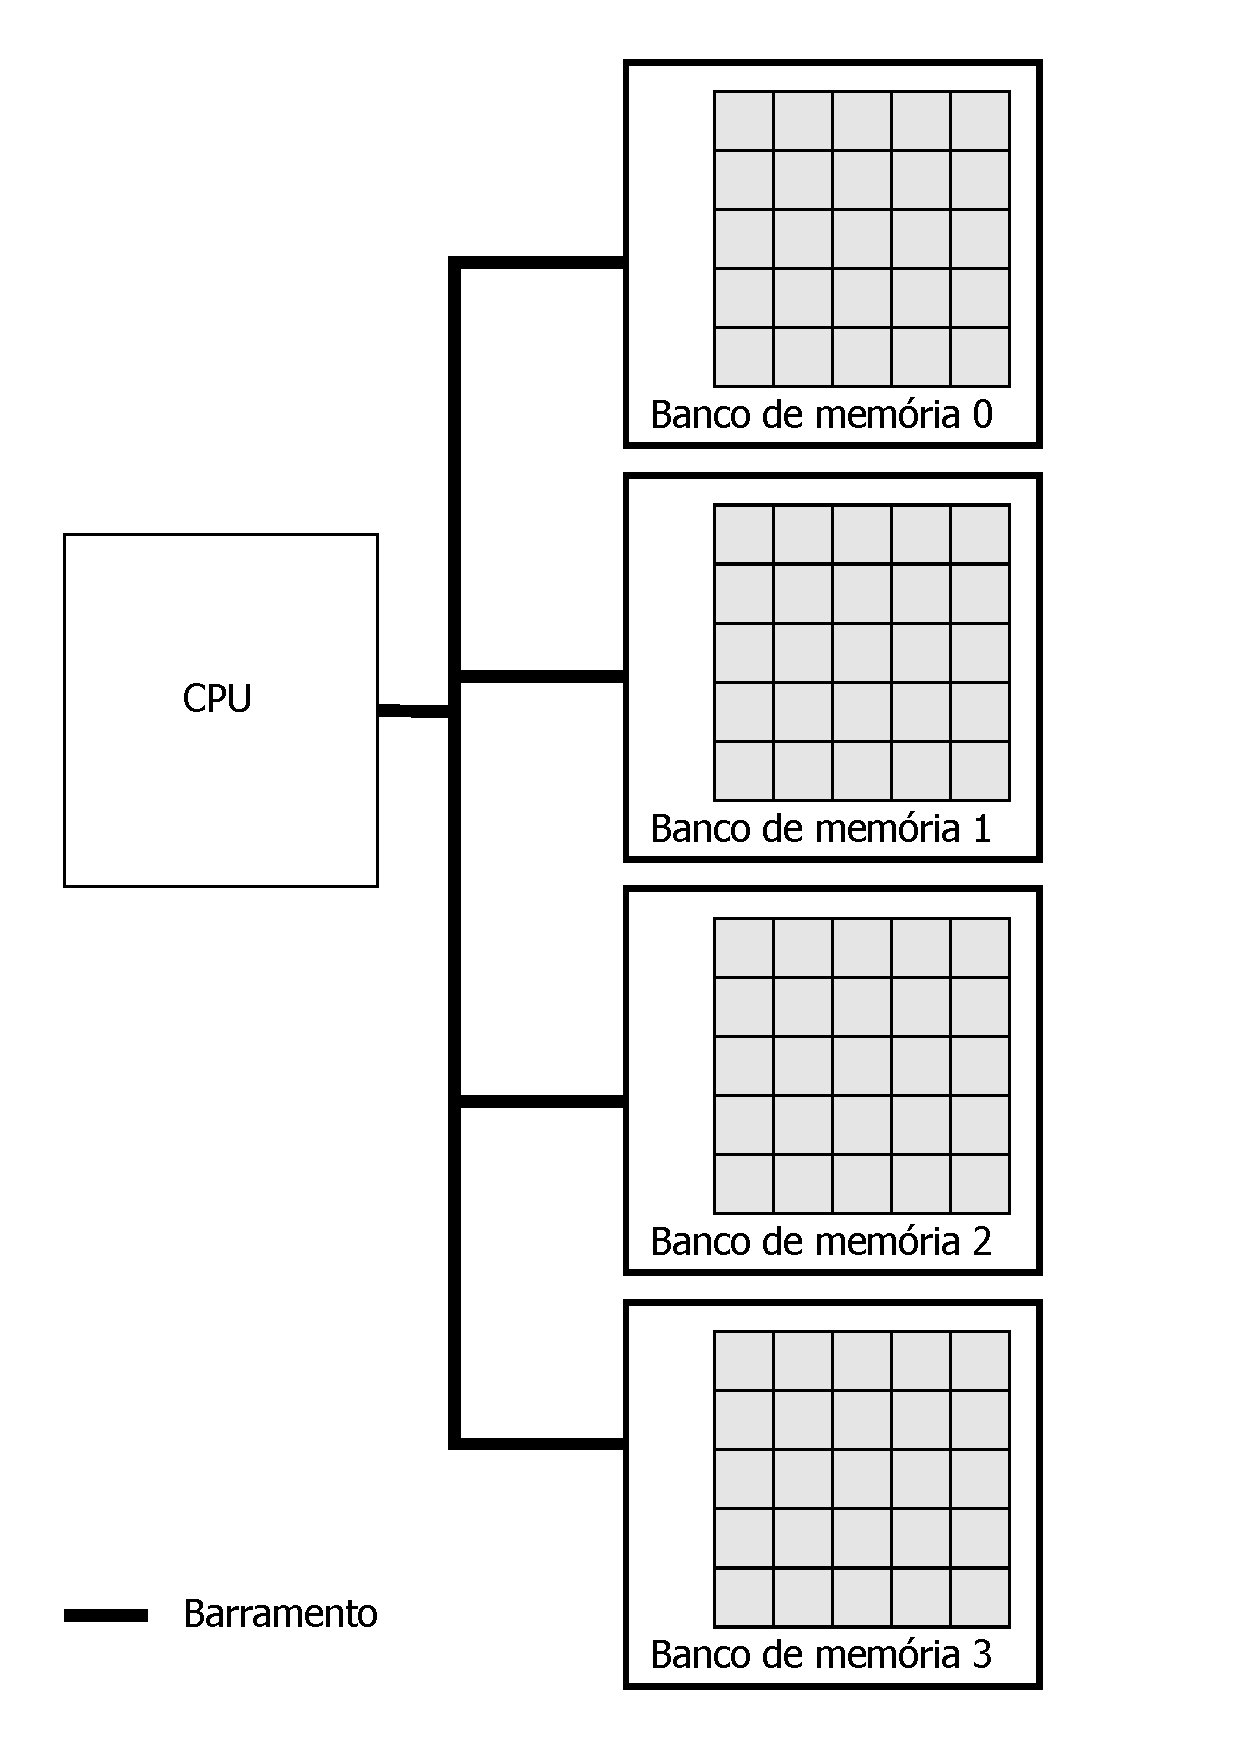
\includegraphics[width = 0.4 \linewidth]{figs/topologia.pdf}}
\subfigure[\label{FIG:MEM_VECTOR}]{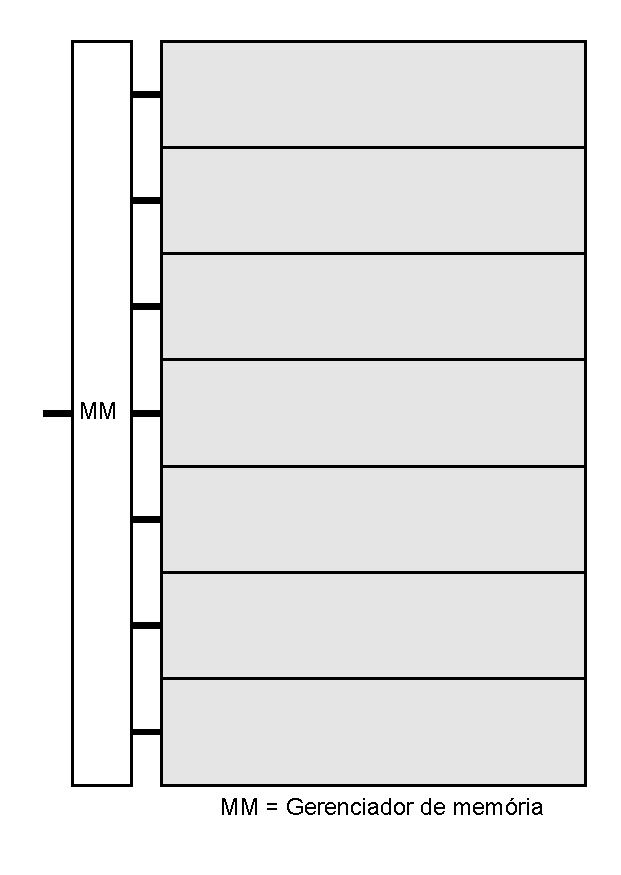
\includegraphics[width = 0.4 \linewidth]{figs/vector.pdf}}
\caption[Topologias da mem�ria]{Topologia da mem�ria como fisicamente disposta (a) e como vista por uma aplica��o (b).} \label{FIG:MEM_TOPOLOGY}
\end{figure}

Al�m disto, por��es fragmentadas da mem�ria f�sica podem ser alocadas para um processo, mas o gerenciador virtualiza estes fragmentos em um espa�o cont�nuo de endere�amento, como ilustrado na Figura \ref{FIG:MEM_VIRTUAL}.

\begin{figure}[!ht]
\centering
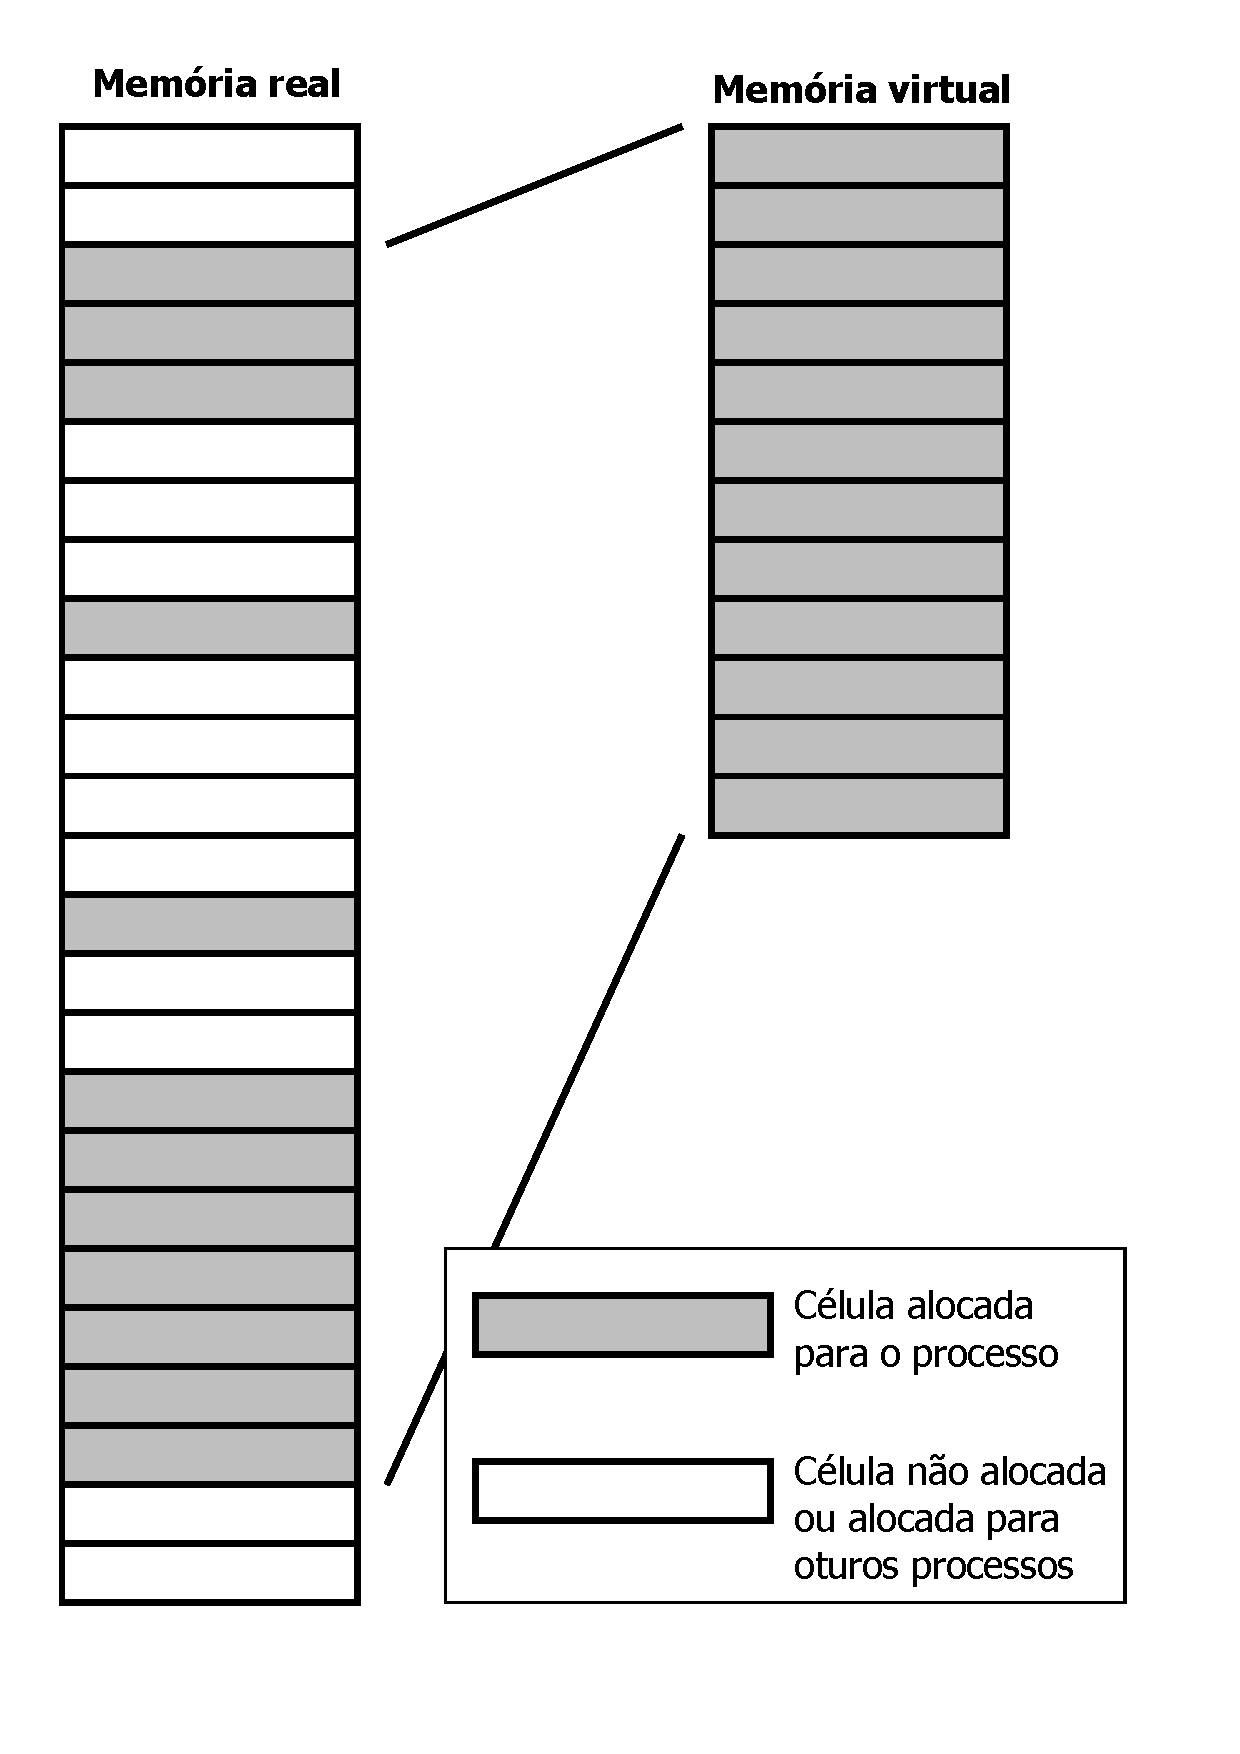
\includegraphics[width = 0.5 \linewidth]{figs/mem_virtual.pdf}
\caption[Mem�ria virtual]{Mem�ria virtual como alocada para um processo (adaptado de \cite{TANENBAUM:2001}).} \label{FIG:MEM_VIRTUAL}
\end{figure}

A pagina��o � outro mecanismo presente nos gerenciadores e est� geralmente associado � mem�ria virtual. Isto faz com que o sistema guarde por��es de dados (p�ginas) da mem�ria principal em uma mem�ria secund�ria, recuperando-as posteriormente quando seu uso for solicitado. Desta forma, o sistema expande a mem�ria virtual dispon�vel para as aplica��es. Geralmente se utiliza como mem�ria secund�ria um espa�o reservado no disco (HD, SSD, etc). Estes dispositivos s�o mais lentos que as \ac{RAM}s mas possuem maior disponibilidade de armazenamento e s�o mais baratos, se levado em conta o valor por byte. \cite{TANENBAUM:2001}

No Linux, o espa�o reservado para pagina��o � chamado de \emph{swap} e pode estar presente ou n�o em um sistema, assim como pode ser habilitado, desabilitado ou redimensionado em tempo de execu��o.

Como o processo de salvar e recuperar as p�ginas do disco � lento, o Linux evita utilizar a �rea de \emph{swap} at� que a disponibilidade de mem�ria livre esteja baixa.

\subsection{Escassez de Mem�ria}

A \ac{OOM} � um estado de um sistema computacional, geralmente indesejado, onde nenhuma mem�ria adicional pode ser alocada para uso pelos programas ou pelo pr�prio sistema operacional.

No caso do Linux, para lidar com este tipo de situa��o � utilizada uma ferramenta, parte do subsitema \ac{LinuxMM}, chamada de OOM \emph{Killer}, que consiste em uma tarefa que sacrifica um ou mais processos para liberar mem�ria para o sistema \cite{OOMKILLER:2009}.

Programas que utilizam muita mem�ria podem esgotar a mem�ria do sistema, fazendo-o deixar de funcionar. Isto pode, por exemplo, levar a uma situa��o em que h� t�o pouca mem�ria que o kernel n�o pode alocar mem�ria para executar uma oper��o de libera��o de mem�ria. Ent�o, neste caso, o OOM Killer � acionado e identifica os processos a serem sacrificados para beneficiar o resto do sistema.

O OOM Killer usa um esquema de pontua��o para decidir qual ou quais processos sacrificar. Os pontos s�o dados pela fun��o \emph{badness}, que utiliza uma f�rmula relativamente simples, documentada no pr�prio c�digo. As regras para gerar a pontua��o s�o:

\begin{itemize}
  \item perder o m�nimo de trabalho realizado;
  \item recuperar a maior quantidade de mem�ria;
  \item n�o matar (\emph{kill}) nada que tenha utilizado pouca mem�ria;
  \item matar o m�nimo de processos (de prefer�ncia apenas um);
  \item tentar matar o processo que o usu�rio espera que v� ser morto (menor surpresa).
\end{itemize}

\subsection{Cache de Mem�ria}

Uma caracter�stica do \ac{LinuxMM} do mecanismo de \emph{cache} de mem�ria. Ele � manipulado pelo Linux Page Cache e funciona da seguinte forma: no Linux, quando um arquivo � acessado, seu conte�do � copiado para a mem�ria para ser trabalhado (lido e/ou escrito); ent�o, quando o processo termina, o \emph{kernel} pode liberar aquela mem�ria ou mant�-la em \emph{cache} para caso algum outro processo o acesse. O mesmo ocorre com algumas outras formas de aloca��o da mem�ria.

Devido ao \emph{cache} em sistemas Linux, ap�s algum tempo de execu��o de processos, apenas uma pequena por��o da mem�ria pode permanecer marcada realmente como livre. A maior parte est� sempre preenchida com conte�do �til, mas nem sempre isso significa que esteja sendo utilizada. Por outro lado h� um ganho de desempenho consider�vel ao acessar recursos recentemente utilizados (em \emph{cache}).

Um conte�do que esteja em \emph{cache} pode ser liberado quando h� uma solicita��o por aloca��o de mem�ria e n�o h� mem�ria livre para atender. Neste caso, o conte�do do \emph{cache} � descartado e a mem�ria � cedida ao processo que solitou a aloca��o. 

\section{Resumo do Cap�tulo}

Este cap�tulo apresentou, de maneira resumida, alguns fundamentos da �rea de testes de mem�ria que s�o �teis para melhor compreens�o deste trabalho, mostrou os v�rios tipos de falhas e testes estudados, dando �nfase nas falhas mais comuns e nos testes de complexidade realiz�vel na tecnologia atual. Tamb�m foram apresentadas algumas caracter�sticas de como o Linux gerencia a mem�ria f�sica do sistema.

No cap�tulo seguinte, ser�o apresentadas as ferramentas utilizadas para o desenvolvimento, teste e valida��o, al�m de detalhes da implementa��o da ferramenta concebida neste trabalho. 